%%%%%%%%%%%%%%%%%%%%%%%%%%%%%%%%%
% Methodology                   %
%%%%%%%%%%%%%%%%%%%%%%%%%%%%%%%%%

\section{Methodology}

This chapter presents the methodological approach adopted for the project and explains how it was applied in practice. It first introduces Design Science Research (DSR) as the overarching research methodology, describing how the method works, why it fits this project, and how it was applied through four iterations. It then presents the Agile development approach used to build the tool and shows how the two are combined. The chapter next describes the project management dimension of the work, the six project phases and their planning, visualized as a Gantt chart in Figure~\ref{fig:gantt}, and the way the phases map onto the iterations. It closes with the stakeholder analysis, the research materials, the research ethics, and the technologies and tools used.

\subsection{Design Science Research}

Design Science Research (DSR) is a methodology widely adopted in information systems research when the objective is to create and evaluate an artifact that solves a practical problem, rather than only to analyze or theorize about it \cite{hevner2004}. Artifacts produced through DSR may take the form of constructs, models, frameworks, methods, or instantiations such as software tools. DSR is therefore best suited to projects that must \emph{build} something to answer their research question, projects that are both analytical and constructive, that address a concrete organizational need, and that improve their solution through repeated cycles of design and evaluation rather than through a single act of analysis. A project whose contribution is a working, evaluated artifact, as opposed to a purely descriptive study, is exactly the kind of project for which DSR was conceived.

\subsubsection{The DSR Regulative Cycle}

DSR structures each iteration through the regulative cycle, which organizes the work into five activities. The first, problem investigation, characterizes the problem the iteration addresses, its stakeholders, and the criteria a satisfactory solution must meet. The second, solution design, defines the artifact or component that is expected to address the problem, together with its underlying design decisions. The third, design validation, checks the design against the requirements and against the knowledge base before significant effort is committed to building it. The fourth, solution implementation, builds the artifact, whether a documented framework component or a piece of the tool. The fifth, solution evaluation, assesses the result against evidence and against the criteria set during problem investigation, and its findings feed the problem investigation of the following iteration.

This five activity structure gives the project a repeatable and auditable rhythm. Because evaluation feeds directly back into the next problem investigation, the framework and the tool are not designed once and frozen, but are progressively corrected as field evidence and regulatory requirements are confronted. For example, a validation finding on the framework, such as the risk that a respondent overstates maturity without proof, is carried forward as a problem to be solved in the following iteration, where it becomes the evidence cap rule implemented in the scoring engine. Figure~\ref{fig:dsr-cycle} illustrates the regulative cycle and its application across the four iterations of the project.

\begin{figure}[H]
\centering
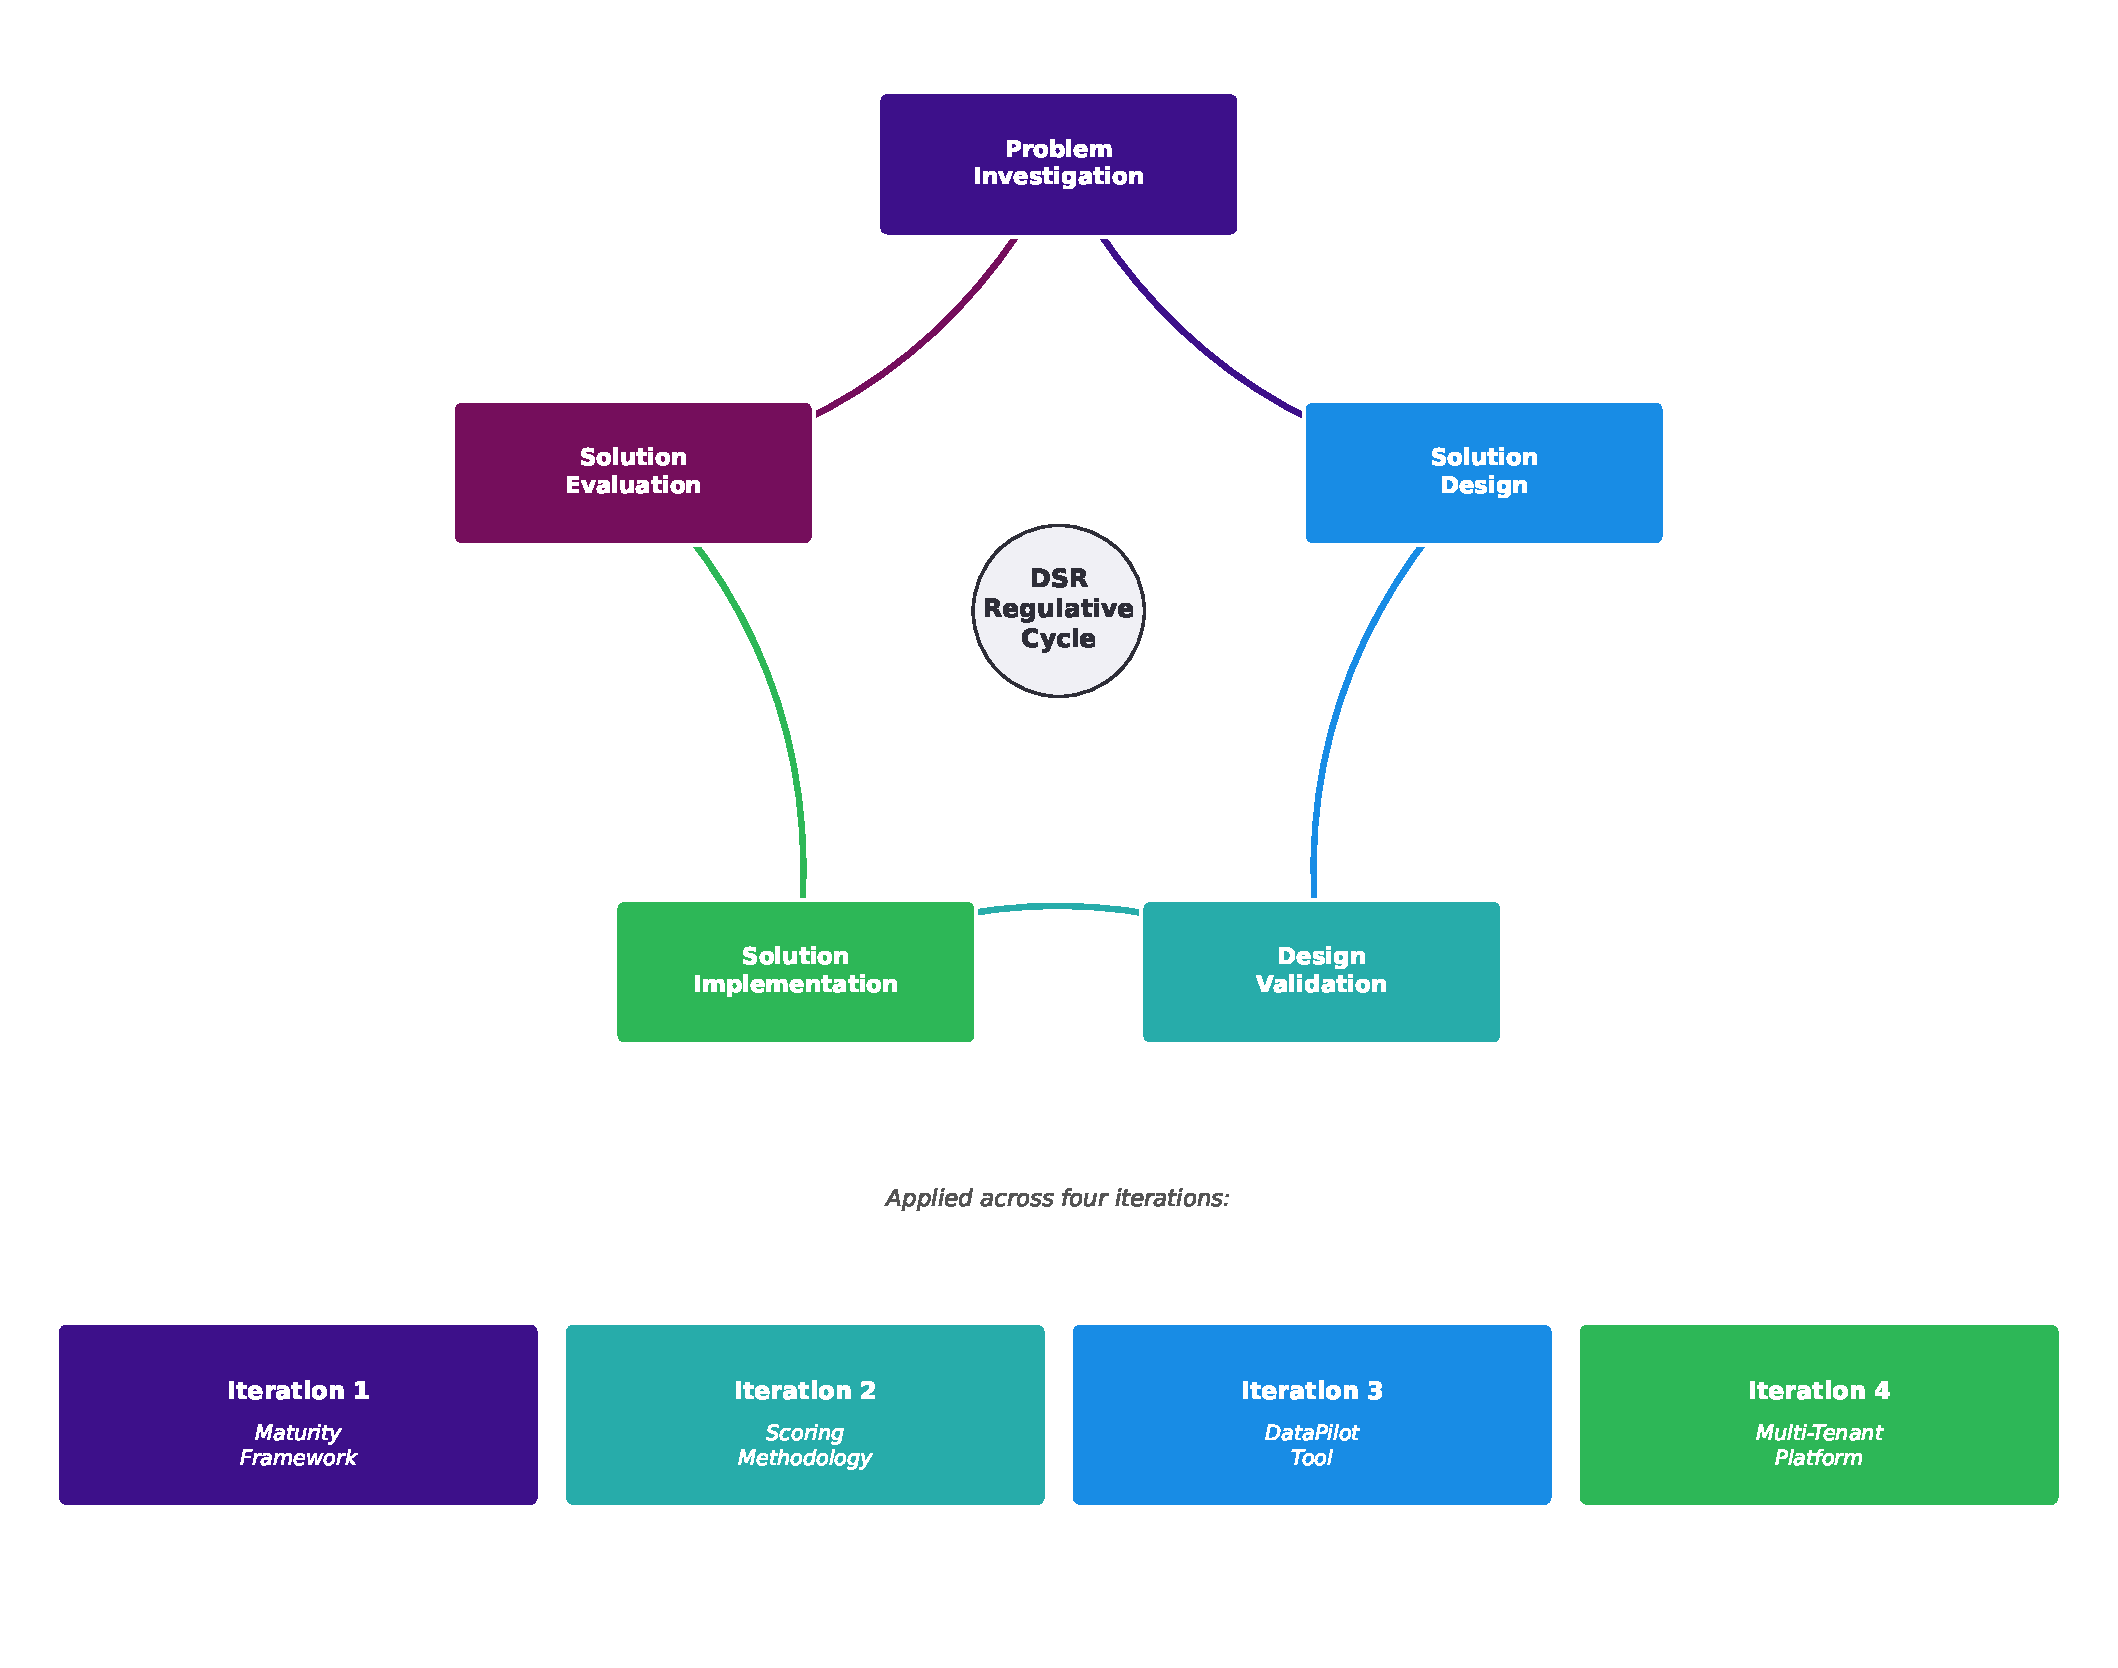
\includegraphics[width=0.85\textwidth]{images/dsr-cycle.pdf}
\caption{The DSR regulative cycle applied across the four iterations}
\label{fig:dsr-cycle}
\end{figure}

\subsubsection{Motivation for Adopting DSR}

This project is well suited to DSR because it is both analytical and constructive. Its central objective is to produce two concrete artifacts, and the problem it addresses, the absence of a sector specific and regulation aligned means of assessing data maturity, is a real organizational challenge faced by banking institutions. Generic maturity models exist, but none of them encodes the specific obligations that a Tunisian bank must satisfy, such as the formal mapping to BCT Circulaire N\textdegree{}2025-08 requirements or the data traceability expected under BCBS 239 for risk reporting. A methodology centered purely on description or theory building would not close this gap, because the gap is the absence of a usable instrument, not the absence of an explanation.

The project produces two closely coupled artifacts, which is precisely what DSR is designed to deliver. The first is a model, the hybrid data maturity assessment framework, comprising five dimensions, twelve sub-dimensions, forty seven indicators, and an associated scoring method. The second is an instantiation, the DataPilot tool, which operationalizes the framework as an interactive single-page web application. The framework is the conceptual contribution, and the tool is the concrete embodiment that makes the framework usable, repeatable, and auditable in a real banking setting. Treating both as designed artifacts allows each to be evaluated on its own terms, the framework for validity and completeness of coverage, and the tool for correctness, usability, and fidelity to the framework.

The choice is further justified by the three design science cycles that connect a design project to its environment and to its knowledge base \cite{hevner2004}. The relevance cycle grounds the project in the environment of the Tunisian banking sector, drawing its requirements from the regulatory drivers, principally BCT Circulaire N\textdegree{}2025-08 and the BCBS 239 principles, and from the diagnostic survey of banking professionals. The design cycle is the inner loop in which the framework and the tool are iteratively built and evaluated. The rigor cycle connects the project to the existing knowledge base, in particular the five established maturity frameworks analyzed in the previous chapter, so that the hybrid model retains what is proven in the state of practice while adding what the sector and its regulation specifically require. The relevance cycle ensures the artifacts solve a real problem, the rigor cycle ensures they are grounded in established knowledge, and the design cycle repeatedly reconciles the two. The methodology also fits the dual academic and industrial nature of a capstone conducted within a professional services environment, since it demands both a rigorous, defensible design rationale and a working deliverable that a practitioner can use.

\subsubsection{Iterative and Incremental Development}

DSR was applied to this project through four iterations, each a complete turn of the regulative cycle that designed, validated, implemented, and evaluated one artifact before the next began. The four iterations follow a single progression that can be named in four words, Define, Measure, Steer, and Scale. Iteration~1 \emph{defines} what data maturity means for a Tunisian bank by fixing the dimensions, sub-dimensions, and indicators against which every institution is assessed. Iteration~2 \emph{measures} that maturity by turning the forty seven indicator scores into a single auditable index. Iteration~3 \emph{steers} by embedding the measurement in an interactive tool. Iteration~4 \emph{scales} the instrument from a single assessor into a role based, tenant isolated platform. Each iteration consumes the validated artifact of its predecessor as its input, so the framework of the first becomes the object measured by the second, the scoring engine of the second becomes the core embedded in the third, and the tool of the third becomes the foundation that the fourth scales into a platform. Table~\ref{tab:dsr-iterations} summarizes the four iterations, stating for each the design question, the solution designed and validated, the artifact implemented, and the outcome of its evaluation. This table is the reference point for the next chapter, where each cell is developed into a full DSR activity subsection.

\begin{table}[H]
\centering

\footnotesize
\setlength{\tabcolsep}{4pt}
\begin{tabular}{|p{0.8cm}|p{3.3cm}|p{3.7cm}|p{2.6cm}|p{3.6cm}|}
\hline
\textbf{Iter.} & \textbf{Problem investigated (design question)} & \textbf{Solution designed and validated} & \textbf{Artifact implemented} & \textbf{Evaluation outcome} \\
\hline
1 & Can the breadth of data management be structured into an assessable hierarchy aligned with the BCT Circulaire N\textdegree{}2025-08 and BCBS 239 requirements? & Hybrid structure of five dimensions, twelve sub-dimensions, and forty seven indicators; dimension weights of 25/20/20/20/15 and the mapping of the regulatory obligations onto indicators validated & Framework catalogue with a five-level rubric per indicator & Coverage of the five areas and regulatory alignment confirmed; Skills and Culture retained as a proxy-only dimension \\
\hline
2 & Can forty seven indicator scores be aggregated into a single auditable index that resists over-optimistic self-assessment? & Weighted, renormalized aggregation chain plus four business rules: the evidence requirement, the anti-gaming evidence cap, the bounded skip logic, and the non-skippable status of the thirteen regulatory indicators & Scoring engine expressed as pure store selectors & Worked example verified by hand: GMI of 2.19/5, displayed as 44\% and Level 2, Emerging; evidence cap confirmed, a score of 4 without evidence computing as 2 \\
\hline
3 & Can the framework and its scoring methodology be operationalized as an interactive tool usable by bank management? & Six-screen client-side single-page application with a completion gate protecting the result screens & The DataPilot tool & Functional testing and simulated assessment scenarios on anonymized data confirmed the fidelity of the tool to the scoring methodology \\
\hline
4 & Can one assessment be produced by many contributors across a bank, under EY oversight, without weakening confidentiality or auditability? & Four-role hierarchy with a top-down invite chain, departments with dimension-to-department assignments, per-bank copies of the EY master template, and two-layer enforcement combining row-level security with service-role endpoints & The DataPilot multi-tenant platform & Functional scenarios on the seeded demo bank confirmed the role gates, the tenant isolation, and the immutability of finalized submissions \\
\hline
\end{tabular}
\caption{Summary of the DSR regulative cycle across the four iterations}
\label{tab:dsr-iterations}
\end{table}

No research question is answered by a single iteration alone. Table~\ref{tab:rq-iterations} makes this explicit by mapping the three research questions of the introduction onto the diagnostic survey and the four iterations. The survey is shown as a distinct column because it belongs to the field diagnostic of Phase~1 and is not itself a DSR iteration; it supplies the evidence against which the designed artifacts are calibrated, whereas the iterations produce those artifacts.

\begin{table}[H]
\centering

\footnotesize
\setlength{\tabcolsep}{4pt}
\begin{tabular}{|p{1.0cm}|p{6.8cm}|c|c|c|c|c|}
\hline
\textbf{RQ} & \textbf{Focus} & \textbf{Survey} & \textbf{Iter. 1} & \textbf{Iter. 2} & \textbf{Iter. 3} & \textbf{Iter. 4} \\
\hline
RQ1 & Current state of data maturity in Tunisian banks and gaps relative to standards and regulatory requirements & X & X & & & \\
\hline
RQ2 & Design of a maturity assessment framework fitted to the Tunisian banking sector & X & X & X & & \\
\hline
RQ3 & Extent to which an interactive steering tool supports decision-making and accelerates transformation & & & X & X & X \\
\hline
\end{tabular}
\caption{Mapping of the research questions onto the survey and the four iterations}
\label{tab:rq-iterations}
\end{table}

The mapping is deliberately honest about where each answer comes from. RQ1 is answered chiefly by the diagnostic survey, with the first iteration supplying the reading grid of dimensions and indicators through which the field evidence is interpreted. RQ2 is answered by the first two iterations, which together produce the framework and the scoring methodology that make it operational, with the survey supplying the field evidence against which the design is calibrated. RQ3 is answered by the second, third, and fourth iterations, since the auditability of the score is a property of the scoring engine, its usability a property of the tool that embeds it, and its deployability across a bank a property of the multi-tenant platform.

\subsection{Agile Development Approach}

While DSR governs the research level of the project, the construction of the tool required a development approach of its own. The tool could not be specified once and built in a single pass: the scoring model and the questionnaire were expected to change as the framework was validated, and the user interface needed continuous testing and refinement. The development therefore followed an iterative and incremental approach in the spirit of Agile, in which the tool was grown as a series of working increments rather than delivered as one monolithic release.

Concretely, and stated honestly, the development did not follow a formal Scrum process with fixed-length sprints, ceremonies, and prescribed roles. It followed the lighter, iterative and incremental discipline that Agile promotes: each iteration of the tool was built as a working increment, exercised against the scoring methodology and against simulated assessment data, and refined before the next increment began, with weekly review meetings steering the direction of the work and surfacing defects and usability problems early. This cadence kept the tool continuously runnable, so that every design decision could be tried in a working build rather than argued on paper, and it allowed the questionnaire, the scoring engine, and the dashboards to stabilize progressively as evidence accumulated.

\subsection{Combining DSR and Agile}

Design Science Research and the Agile development approach operate at two different levels and are combined deliberately rather than merged. DSR governs the research level, providing the rationale for the artifacts, the validation against requirements, and the evaluation against evidence, so that each design decision can be justified and traced. Agile governs the construction level, providing the short, feedback driven cadence through which the scoring engine and the six screens are built and refined. The two are compatible because the DSR design cycle is itself iterative, and each turn of that cycle can be realized as one or more development increments that deliver a working, testable slice of the tool.

Concretely, the four project iterations map onto the DSR design cycle, and the development inside each iteration is organized incrementally. Within an iteration, the five DSR activities set the goals and the acceptance criteria, while the iterative development cadence of planning, building, testing, and refinement produces and stabilizes the increment. The DSR solution evaluation activity and the development testing and refinement steps reinforce each other, since a defect or usability problem surfaced during development is both a testing outcome and evidence that feeds the next problem investigation. This division of labor keeps the research disciplined and the engineering responsive without forcing either concern to imitate the other.

\subsection{Project Phases and Planning}

Beyond the research and development methodologies, the project itself was conducted as a structured consulting engagement over a 24-week plan at EY Tunisia. The work was organized into six phases, a framing phase numbered~0 followed by five delivery phases numbered~1 to~5. Phases~0 to~3 constitute the pre-coding intellectual work of the project, in which the problem is framed, the existing situation analyzed, the needs identified, and the hybrid framework designed, while phases~4 and~5 cover the build and the deployment of the DataPilot tool. The project started on 2~February 2026 with the framing phase, the kickoff presentation was delivered on 12~February 2026, development of the tool began on 11~May 2026, and the project closed with the deployment phase ending on 31~July 2026. In addition to the six phases, a transversal workstream covered report writing, risk management, and project steering with weekly meetings throughout the engagement. Figure~\ref{fig:phases-overview} gives an overview of the six phases, and Table~\ref{tab:project-phases} details, for each phase, its period, its focus and key tasks, and its key deliverables.

\begin{figure}[H]
\centering
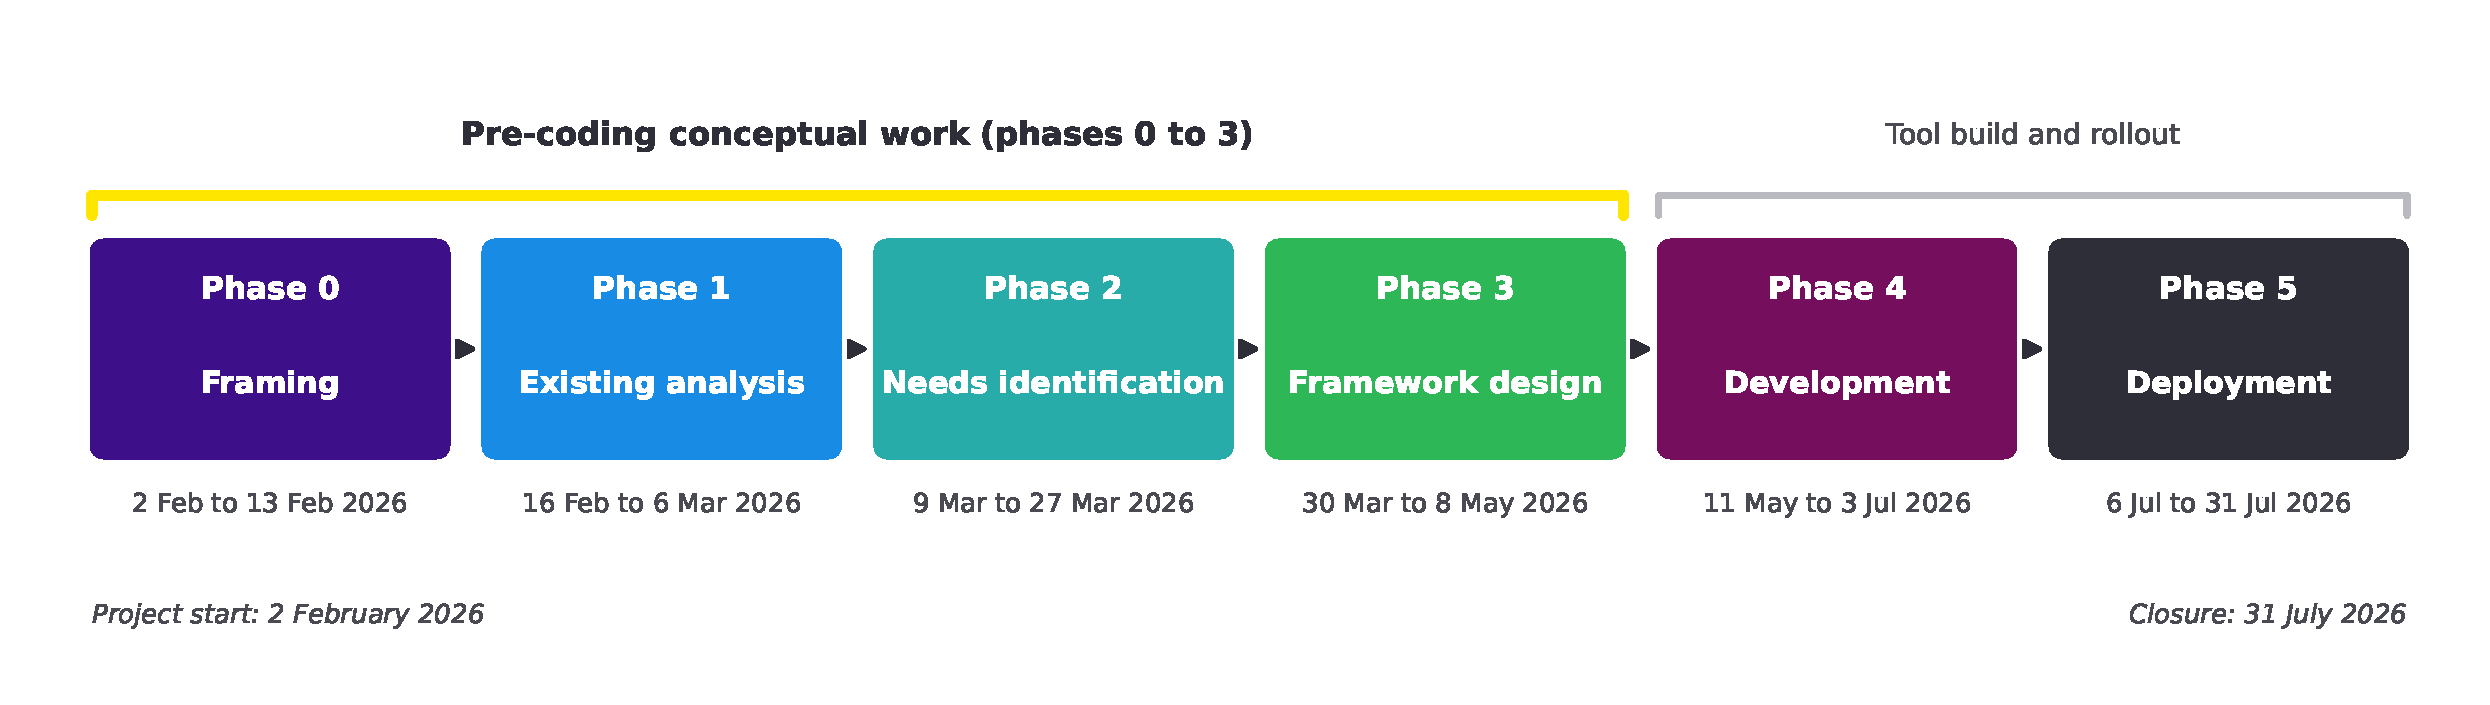
\includegraphics[width=0.95\textwidth]{images/phases-overview.pdf}
\caption{The six project phases from framing to deployment}
\label{fig:phases-overview}
\end{figure}

\begin{landscape}
\begin{table}[H]
\centering

\footnotesize
\setlength{\tabcolsep}{4pt}
\begin{tabular}{|p{2.6cm}|p{3.0cm}|p{10.2cm}|p{6.4cm}|}
\hline
\textbf{Phase} & \textbf{Period} & \textbf{Focus and key tasks} & \textbf{Key deliverables} \\
\hline
Phase 0: Framing & 2 to 13 February 2026 & Team integration; project scoping; benchmark and documentary research; methodology definition; project plan; kickoff preparation and presentation & Methodology document, project plan, kickoff presentation (L6) \\
\hline
Phase 1: Analysis of the existing situation & 16 February to 6 March 2026 & Stakeholder cartography; operational review; conceptual review; identification of limits and risks & Stakeholder map (L1); existing-situation analysis report (L2) \\
\hline
Phase 2: Needs identification & 9 to 27 March 2026 & Study of existing maturity frameworks; business and data needs analysis; functional and analytical requirements; target vision definition & Requirements specification (L3); target solution description (L4) \\
\hline
Phase 3: Framework design & 30 March to 8 May 2026 & Dimensions and maturity levels; scores and indicators; scoring methodology construction; benchmark against market best practice & Data maturity framework (L5); methodological documentation (L6) \\
\hline
Phase 4: Development & 11 May to 3 July 2026 & Development environment setup; questionnaire implementation; dashboard design; automatic maturity calculation; functional and non-regression tests; scenario and business-gain simulation & Interactive steering tool (L7); functional documentation (L8) \\
\hline
Phase 5: Deployment & 6 to 31 July 2026 & Final deployment and validation; results and maturity-gap analysis; final restitution and project closure & Evaluation results (L9); executive presentation (L10); final report (L11) \\
\hline
Transversal & 16 February to 31 July 2026 & Report writing; risk management; project steering and weekly meetings & Continuous steering; final report (L11) \\
\hline
\end{tabular}
\caption{The six project phases: period, focus, and key deliverables}
\label{tab:project-phases}
\end{table}
\end{landscape}

The overall schedule that results from these phases is visualized as a Gantt chart in Figure~\ref{fig:gantt}. Of the planned tasks, the scenario and business-gain simulation was realized in the delivered tool as target-level setting and gap-to-target visualization, with the quantitative what-if simulation of business gains identified as future work, as stated in the results and the conclusion.

\begin{figure}[H]
\centering
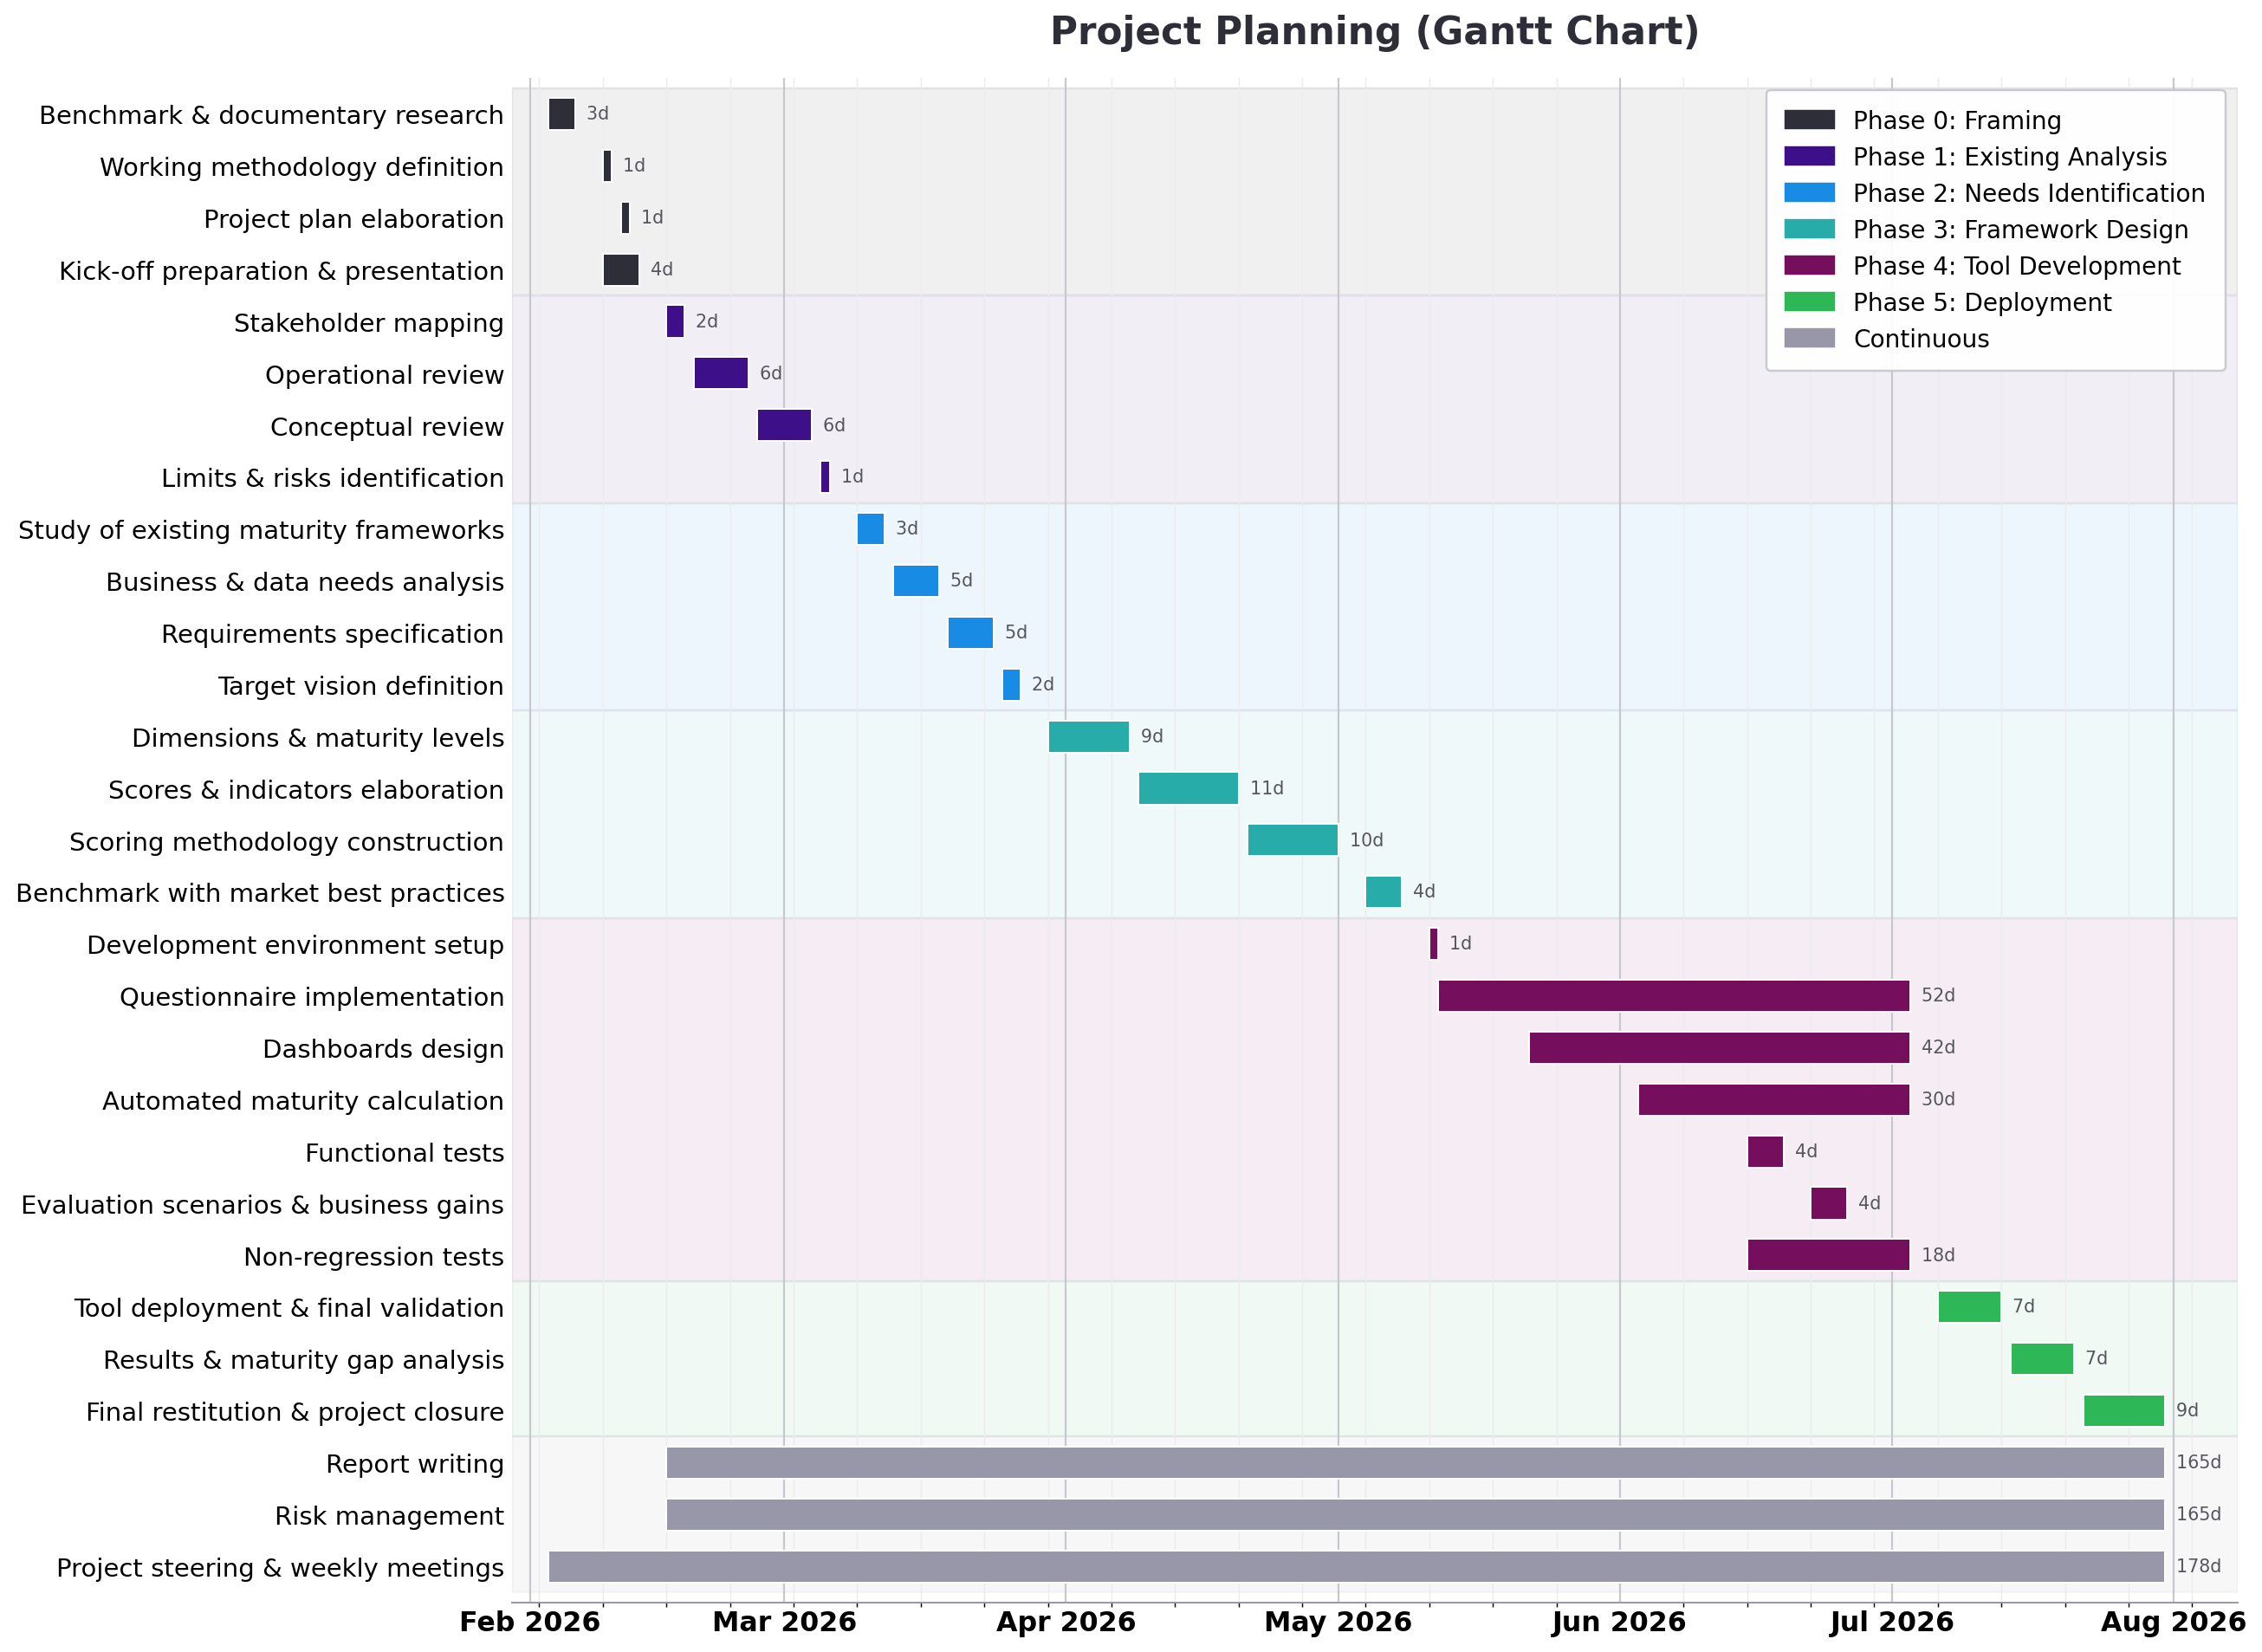
\includegraphics[width=\textwidth]{images/gantt-planning.png}
\caption{Project planning (Gantt chart)}
\label{fig:gantt}
\end{figure}

Across the six phases, eleven deliverables were planned and labeled L1 to L11, listed in Table~\ref{tab:deliverables}. Deliverables L1 to L6 belong to the pre-coding phases~0 to~3, in which the diagnosis, the requirements, and the framework are produced, whereas L7 to L11 are produced during the development and deployment phases~4 and~5, in which the tool is built, evaluated, and handed over.

\begin{table}[H]
\centering
\footnotesize
\setlength{\tabcolsep}{4pt}
\begin{tabular}{|c|p{8.4cm}|p{3.8cm}|}
\hline
\textbf{Code} & \textbf{Deliverable} & \textbf{Produced in} \\
\hline
L1 & Stakeholder mapping & Phase 1 \\
\hline
L2 & Existing-situation analysis report & Phase 1 \\
\hline
L3 & Requirements specification & Phase 2 \\
\hline
L4 & Target solution description & Phase 2 \\
\hline
L5 & Data maturity framework & Phase 3 \\
\hline
L6 & Methodological documentation & Phases 0 and 3 \\
\hline
L7 & Interactive steering tool (DataPilot), extended into the multi-tenant platform & Phase 4 \\
\hline
L8 & Functional documentation & Phase 4 \\
\hline
L9 & Evaluation results & Phase 5 \\
\hline
L10 & Executive presentation & Phase 5 \\
\hline
L11 & Final report & Phase 5 \\
\hline
\end{tabular}
\caption{The eleven project deliverables (L1 to L11)}
\label{tab:deliverables}
\end{table}

The six phases and the four DSR iterations are two complementary views of the same work: the phases give the project management timeline of \emph{when} each block of work was done, while the iterations give the research and engineering logic of \emph{what} was designed and evaluated. Table~\ref{tab:phase-iteration-map} makes the correspondence explicit, mapping each phase to the iteration or iterations it carries and to the deliverables it produces. The pre-coding phases carry Iteration~1 and begin Iteration~2, while the build and deployment phases carry Iterations~2 to~4.

\begin{table}[H]
\centering

\footnotesize
\setlength{\tabcolsep}{4pt}
\begin{tabular}{|p{4.2cm}|p{4.6cm}|p{5.4cm}|}
\hline
\textbf{Phase} & \textbf{DSR iteration(s)} & \textbf{Deliverables} \\
\hline
Phase 0: Framing & Project setup (pre-iteration) & L6 \\
\hline
Phase 1: Existing situation & Iteration 1 (Define) & L1, L2 \\
\hline
Phase 2: Needs identification & Iteration 1 (Define) & L3, L4 \\
\hline
Phase 3: Framework design & Iteration 1 (Define); begins Iteration 2 (Measure) & L5, L6 \\
\hline
Phase 4: Development & Iterations 2 (Measure), 3 (Steer), 4 (Scale) & L7, L8 \\
\hline
Phase 5: Deployment & Iterations 3 (Steer), 4 (Scale) & L9, L10, L11 \\
\hline
\end{tabular}
\caption{Mapping of the project phases to the DSR iterations and deliverables}
\label{tab:phase-iteration-map}
\end{table}

\subsection{Stakeholder Analysis}

Because the framework and the tool are intended to be used inside banking institutions within an advisory engagement, a stakeholder analysis was conducted during Phase~1 to identify who is affected by a data maturity assessment, what each actor expects from it, and how each actor should be engaged. It is useful to separate two groups whose involvement in this project is of a different nature. The first group is made of the stakeholders who were \emph{actually involved} in producing the work, the EY mission team within which the project was carried out, listed in Table~\ref{tab:stakeholders-ey}: the EY Partner, the Engagement Manager, the project team of consultants that includes the author of this report, and the sector experts consulted for banking and regulatory relevance. The academic and institution supervisors steer the work alongside this team. The second group, in Table~\ref{tab:stakeholders-bank}, is made of the internal stakeholders of a client bank, the roles for whom the instrument is designed and who would be engaged when the assessment is run inside an institution; in the present project, conducted at EY and evaluated on simulated data, these are prospective users rather than participants.

\begin{table}[H]
\centering

\footnotesize
\setlength{\tabcolsep}{4pt}
\begin{tabular}{|p{3.0cm}|p{4.6cm}|p{6.9cm}|}
\hline
\textbf{Stakeholder} & \textbf{Role} & \textbf{Interest} \\
\hline
EY Partner & Global responsibility for the mission & Commercial performance and reputation \\
\hline
Engagement Manager & Operational steering of the mission & Respect of deadlines, quality, deliverables \\
\hline
Project team (consultants) & Interviews, scoring, analysis, and development of the artifacts & Sound methodological execution and a working deliverable \\
\hline
Sector experts & Banking and regulatory expertise input & Guarantee regulatory relevance \\
\hline
\end{tabular}
\caption{Stakeholders of the EY mission (the project's own stakeholders)}
\label{tab:stakeholders-ey}
\end{table}

\begin{table}[H]
\centering

\footnotesize
\setlength{\tabcolsep}{4pt}
\begin{tabular}{|p{3.0cm}|p{4.6cm}|p{6.9cm}|}
\hline
\textbf{Stakeholder} & \textbf{Role} & \textbf{Interest} \\
\hline
Chief Data Officer & Responsible for data governance & Steer the transformation plan and track the evolution of the maturity level \\
\hline
Data Manager & Operational coordination of data management & Structure improvement initiatives and strengthen data processes \\
\hline
Data Owners & Owners of business data & Improve the quality, traceability, and reliability of data in their scope \\
\hline
Risk Manager & Supervision of data-related risks & Ensure control of operational and regulatory data risks \\
\hline
IT Manager & Management of infrastructure and information systems & Anticipate the technical and budgetary impacts of recommendations \\
\hline
Data Architect & Design of the target data architecture & Align the architecture with expected maturity standards \\
\hline
Compliance Officer & Guarantor of regulatory compliance & Verify the alignment of the data mechanism with regulatory requirements \\
\hline
Internal Audit & Independent control of the mechanism & Evaluate the effectiveness of the data governance framework and action plans \\
\hline
Governing body / Board & Strategic sponsor and budget decision-maker & Obtain a consolidated view of data maturity to orient strategy and prioritize investments \\
\hline
\end{tabular}
\caption{Internal stakeholders of a client bank (the instrument's target users)}
\label{tab:stakeholders-bank}
\end{table}

To plan engagement, the stakeholders of both groups were positioned on an interest and influence matrix, shown in Figure~\ref{fig:stakeholder-matrix}. The matrix is a classic stakeholder management tool: it places each actor on two axes, the interest the actor has in the outcome and the influence the actor can exert on it, and the resulting quadrant prescribes an engagement strategy, manage closely, keep satisfied, keep informed, or simply monitor. Its role in this project is to decide where attention and communication effort should be concentrated. The actors combining high interest and high influence, namely the Chief Data Officer, the governing body or board, the EY Partner, the Engagement Manager, and the project team, fall in the \emph{manage closely} quadrant, since they both drive the assessment and act on its results. The remaining actors were positioned according to their respective interest and influence and are to be kept satisfied, kept informed, or monitored. The author of this report sits inside the project team, in the high interest and high influence quadrant: as the consultant who designs the framework, builds the tool, and reports the findings, the author is both a producer of the assessment and directly accountable for its methodological soundness, which places the author among the actors to be managed most closely. The resulting stakeholder cartography constitutes deliverable~L1 and was presented in the weekly meeting of 24~February 2026.

\begin{figure}[H]
\centering
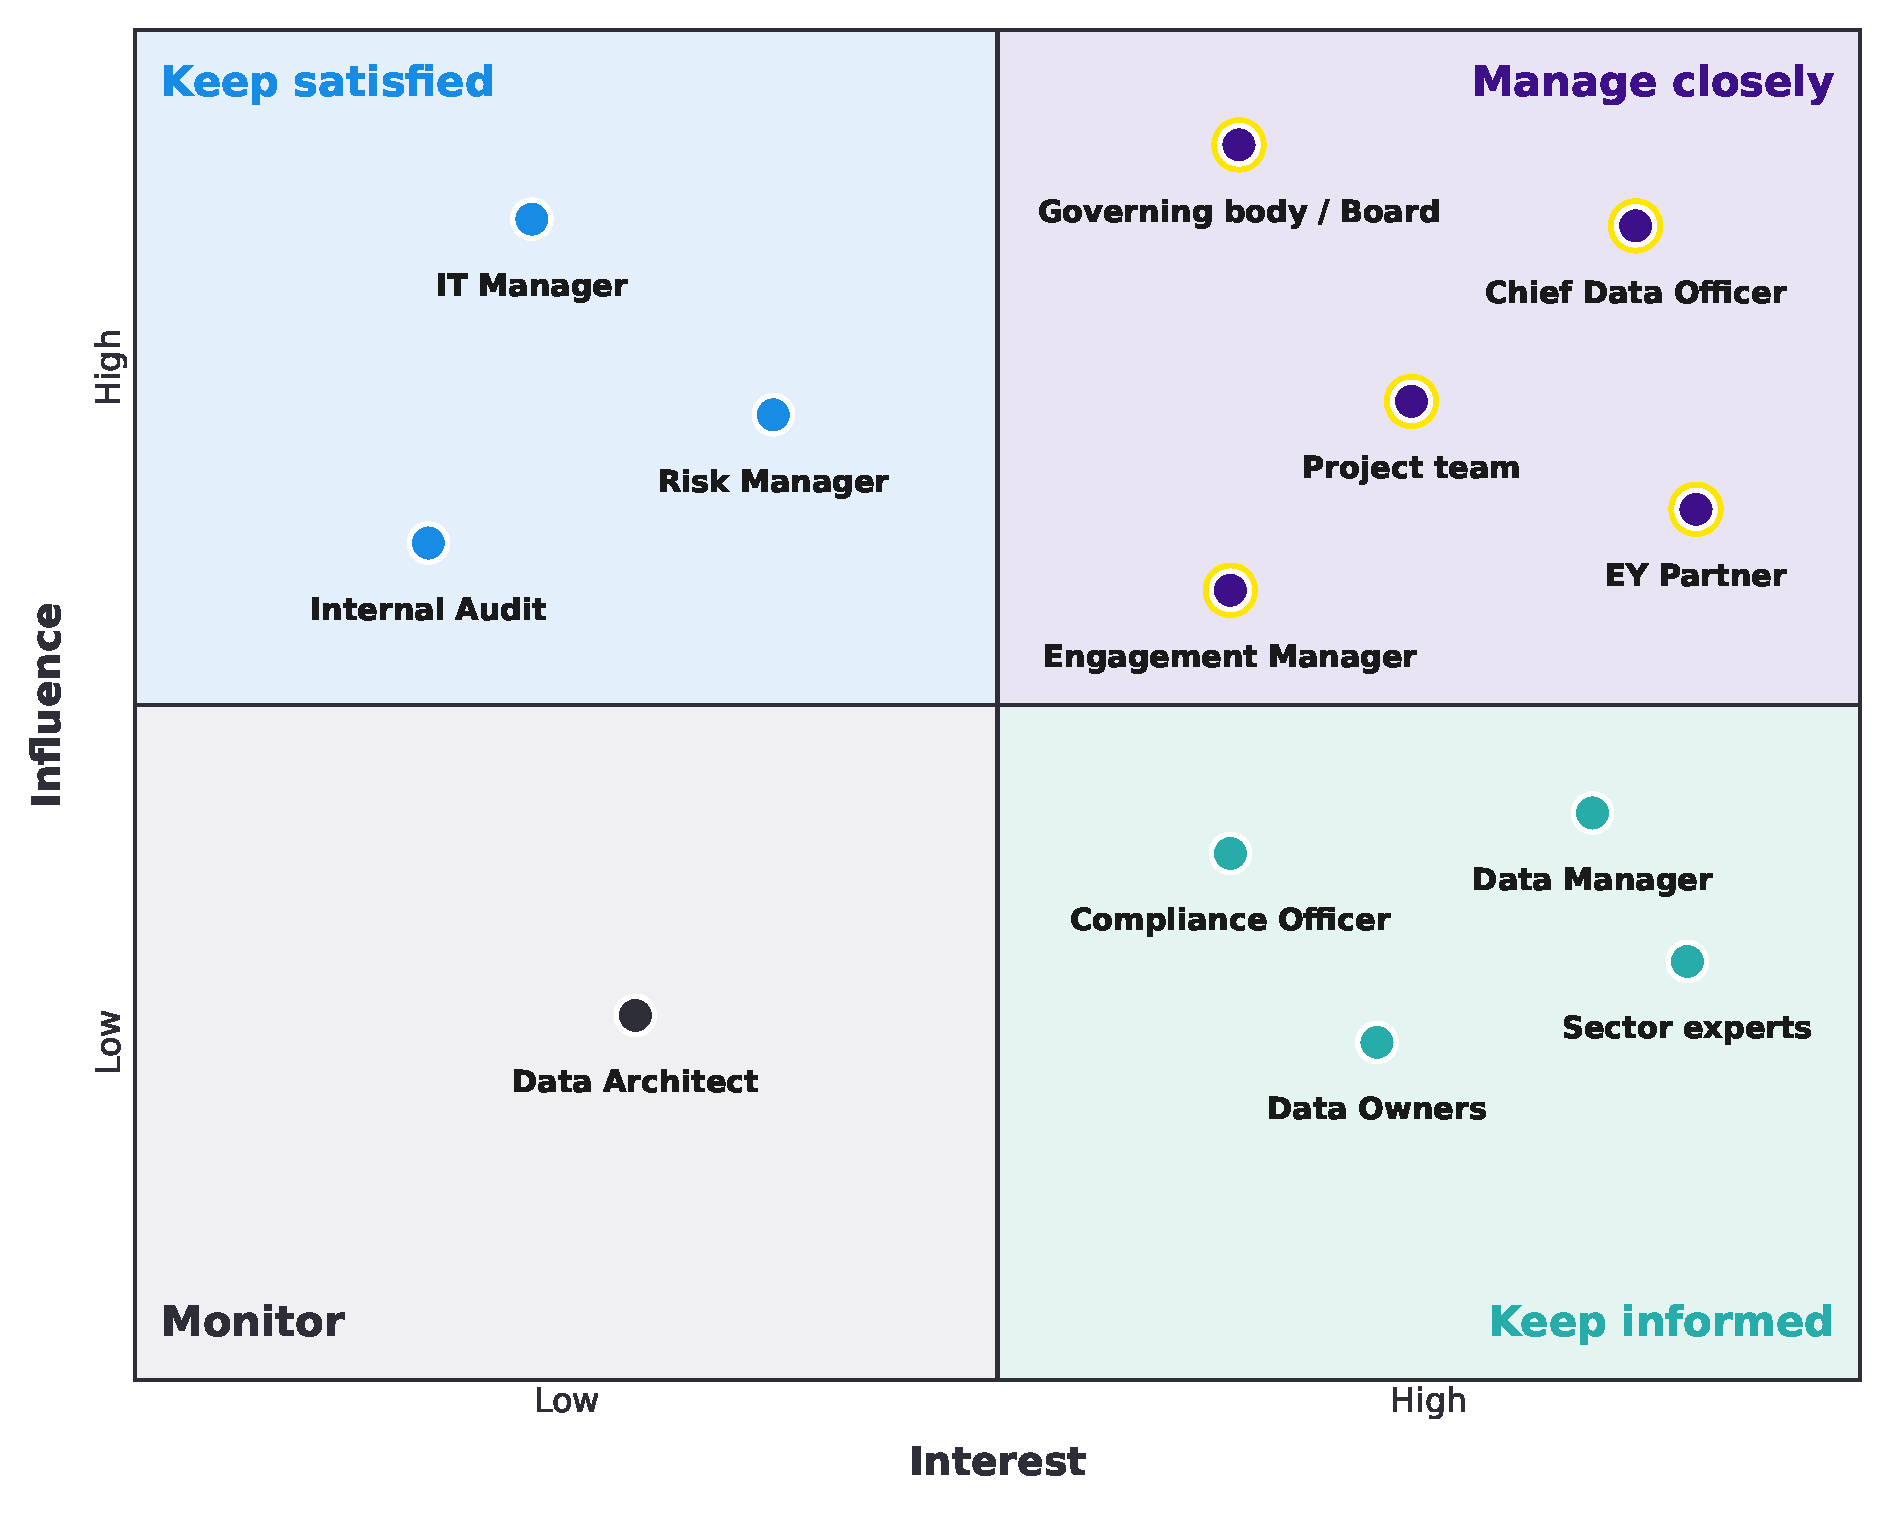
\includegraphics[width=0.8\textwidth]{images/stakeholder-matrix.pdf}
\caption{Stakeholder interest and influence matrix}
\label{fig:stakeholder-matrix}
\end{figure}

\subsection{Research Materials}

The design of the framework is grounded in two categories of research materials, both gathered during the pre-coding phases. The first is the diagnostic survey of 44 banking professionals, conducted as part of the Phase~1 analysis of the existing situation, which provides the field evidence on the current state of data governance, quality, architecture, analytics, and culture in the sector, and which informs both the diagnosis and the calibration of the framework. The second is a benchmark that screened fifteen international data maturity frameworks and retained five, DAMA-DMBOK, DCAM, CMMI-DMM, TDWI, and Gartner, whose comparative analysis, presented in the previous chapter, determines the role retained from each in the hybrid model.

The diagnostic survey is the principal source of field evidence for the relevance cycle and is best understood as the Phase~1 diagnostic that precedes the design iterations. It was administered to 44 professionals working in the Tunisian banking sector, in roles connected to data such as data management, information technology, risk, compliance, and analytics functions, so that the responses reflect the perspective of practitioners who deal with the sector data challenges directly. The survey serves two purposes at once. It establishes the diagnosis of the current state of the sector across the areas that the framework covers, and it informs the calibration of the framework by revealing which questions discriminate between organizations and where practices are weakest. The instrument is organized around the same five areas that structure the framework, governance, data quality, architecture and access, analytics and tools, and skills and culture, so that a weakness observed in a given area maps cleanly onto the corresponding dimension, sub-dimension, and indicators. The questions were phrased so that answers describe observable practices rather than opinions, which supports the later principle, embodied in the tool, that a claimed level of maturity must be backed by evidence.

Several limitations of the survey are acknowledged and shape how its results are used. The sample of 44 respondents is modest and was gathered by reaching professionals who were accessible during the project, so it is not a strict probability sample of the sector and the findings are indicative rather than statistically representative. Responses are self reported, which introduces the risk that respondents present their organization more favorably than the underlying practices warrant, a risk that the framework mitigates through the evidence cap applied in the scoring engine. The skills and culture dimension is particularly difficult to observe directly, which is why it is assessed through proxy indicators only. For these reasons the survey is treated as a diagnostic and calibration input, not as a validation of the framework, and the numeric results reported in the results chapter are interpreted with these constraints in mind.

\subsection{Research Ethics and Data Handling}

Because the diagnostic survey involves human participants and the tool records evidence describing internal banking practices, the project applies a set of ethical and data handling principles consistent with the confidentiality expectations of the sector and of the host organization. Participation in the survey was voluntary, and responses were used solely for the purposes of the diagnosis and the calibration of the framework. Results are reported in aggregate across the sector rather than attributed to any named institution or individual, so that no single bank or respondent can be identified from the figures presented in the results chapter.

The design of the tool reinforces this posture, and the mechanism evolved with the tool. In the single-user build of the third iteration, DataPilot ran entirely in the browser and persisted all assessment data only in the local storage of the user browser, so that nothing left the assessing institution's machine. In the delivered platform, in-progress solo answers still remain in the assessor's browser under the key \texttt{datapilot-assessment}, but submitted results, group assessments, user profiles, and per-bank questionnaire copies are stored in the platform's Postgres database, where row-level security confines every row to its own bank, with EY oversight excepted by design. Access to the platform is invite-only with no public sign-up, submissions are immutable once recorded, and the evidence fields are still intended to reference internal documents rather than to reproduce them, which limits the exposure of confidential material within the tool. The confidentiality argument thus rests on tenant isolation enforced in the database rather than on local custody alone, and these measures align the research with the confidentiality obligations of a banking engagement.

\subsection{Technologies and Tools}

This section lists the technologies and tools used in the project, separating the supporting tools of the engagement, used to manage and document the work, from the technologies that make up the DataPilot stack.

\subsubsection{Tools}

The framework and its documentation were produced with standard office and modeling tools, and the diagnostic survey was collected and analyzed with a spreadsheet based workflow. The project planning was managed through a Gantt based schedule. The development of the tool was managed with Git for version control, with the codebase hosted on GitHub in the \texttt{ZizouX0/datapilot\_EY} repository, where changes were developed on dedicated branches and integrated through pull requests. Dependencies were managed with the npm package manager, code quality was enforced with ESLint configured with the React Hooks and React Refresh plugins, and the application was built and served during development with the Vite toolchain.

\subsubsection{Technologies}

The DataPilot tool is implemented as a single-page web application, and each technology in its stack was chosen for a specific reason rather than by default. The front end is built with React~19\footnote{\url{https://react.dev}}, chosen because its component model matches an application made of many small, reusable interface pieces, the indicator rows, the badges, the charts, and because its large ecosystem reduces the risk of a dependency being abandoned. The application is bundled with the Vite~8 build tool\footnote{\url{https://vitejs.dev}}, chosen for its fast development server and its native support for route based code splitting. Navigation between the screens is handled with React Router~7\footnote{\url{https://reactrouter.com}}, using that code splitting so that each screen and its chart dependencies are loaded on demand, which keeps the initial load light. The application state is managed with Zustand~5\footnote{\url{https://zustand.docs.pmnd.rs}}, chosen over heavier alternatives because it lets the scoring logic be expressed as plain, testable selector functions kept separate from the interface; the state is organized as eight stores, and a solo assessment in progress is persisted to the browser local storage so that it survives page reloads. The user interface is styled with Tailwind CSS~4\footnote{\url{https://tailwindcss.com}}, chosen for consistent, utility based styling without a separate stylesheet to maintain. The data visualizations are produced with Recharts~3\footnote{\url{https://recharts.org}}, a charting library built for React that supplies the radar and bar charts of the dashboards, and the report export is handled with react-to-print~3\footnote{\url{https://github.com/MatthewHerbst/react-to-print}}, chosen because it produces a faithful printable version of the dashboards without a server. The fourth iteration extends this front end stack, otherwise unchanged, with a backend built on Supabase\footnote{\url{https://supabase.com}}, chosen because it provides, in one managed service, the Postgres database that holds all tenant data under row-level security, the invite based authentication, and file storage, which is exactly the thin backend a multi-tenant deployment needs. The database is reached from the browser through the Supabase JavaScript client~2 under the public key, while a small set of serverless functions carries the privileged operations that must not be possible from the browser. The application chrome is fully bilingual, English and French, through a hand-rolled internationalization layer, and the language preference follows the user across devices. Table~\ref{tab:tech-stack} summarizes this stack, associating each component of the application with the technology that implements it and the role it plays in the tool.

\begin{table}[H]
\centering

\footnotesize
\setlength{\tabcolsep}{4pt}
\begin{tabular}{|p{3.4cm}|p{3.2cm}|p{7.6cm}|}
\hline
\textbf{Component} & \textbf{Technology} & \textbf{Role in DataPilot} \\
\hline
User interface framework & React 19 & Component based construction of the application screens \\
\hline
Build tool & Vite 8 & Development server and production build of the application \\
\hline
Navigation & React Router 7 & Routing between the screens with route based code splitting \\
\hline
State management & Zustand 5 & Central stores (eight) holding session, questionnaire content, and assessment state; the solo assessment persists to browser local storage under the key \texttt{datapilot-assessment} \\
\hline
Styling & Tailwind CSS 4 & Utility based styling of the user interface \\
\hline
Data visualization & Recharts 3 & Radar chart and dimension bar charts of the dashboards \\
\hline
Report export & react-to-print 3 & Printable version of the dashboards \\
\hline
Backend platform & Supabase & Postgres database with row-level security for tenant data, authentication with invite emails, and file storage \\
\hline
Backend access & Supabase JS client 2 & Database and authentication calls from the browser under the public key and row-level security \\
\hline
Privileged operations & Serverless functions (\texttt{api/}) & Invitations, role and account management, and department assignment, holding the server-only service key \\
\hline
Internationalization & Hand-rolled EN/FR dictionary & Bilingual English and French application and report chrome; the language preference follows the user across devices \\
\hline
\end{tabular}
\caption{Technology stack of the DataPilot tool}
\label{tab:tech-stack}
\end{table}

Beyond the individual choices, the stack was selected for the way it keeps the scoring logic separable from the presentation. The client-side single-page architecture was chosen in the third iteration because, at that stage, it kept the assessment data local to the user machine and avoided the need for a back end server; the architecture is retained in the platform because React with a lightweight state store such as Zustand keeps the scoring logic, the aggregation chain, the evidence cap, the skip logic, and the renormalization, expressed as pure selectors that can be reasoned about and tested independently of the user interface. Extracted into a pure function module, the scoring engine is shared unchanged by the solo and the group assessment paths, so both compute their scores identically and remain faithful to the methodology of the second iteration. The fourth iteration then adds a deliberately thin backend, introduced for multi-tenant isolation: the database itself enforces tenant isolation and role scope through row-level security policies, while the small set of serverless endpoints performs only the operations that must not be possible from the browser, and the role-gated endpoints among them re-check the caller's role against the database on every request. This division preserves the separation between the scoring logic and the presentation, which is what allows the same engine to feed the results, the gap analysis, the compliance screens, and the group assessment finalization consistently.

\subsection{Conclusion}

This chapter presented the combined methodological approach of the project, Design Science Research for the design and validation of the artifacts and an iterative, Agile inspired approach for the development of the tool, together with the project phases and planning, the stakeholder analysis, the research materials, and the technologies used. The next chapter presents the four iterations through which the artifacts were produced.
